\documentclass{article}
\usepackage[utf8]{inputenc}
\usepackage[margin=1.0in]{geometry}
\usepackage{algorithm}
\usepackage[noend]{algpseudocode}
\usepackage{caption}
\usepackage{graphicx}
\usepackage{wrapfig}
\usepackage{amsmath}
\usepackage[makeroom]{cancel}


\title{Image Pyramids and Quadtrees}
\author{Alexey Didenkov \& Neal Bayya}
\date{November 14, 2018}

\begin{document}

\maketitle

\section{Quadtrees}

\subsection{Introduction}
If you recall, last week we talked about Region segmentation, focusing on how to extract and separate regions in images. Back then, our final output was represented pixel-wise, meaning that at every pixel location, we stored the value of the corresponding region. As it turns out, \textbf{quadtrees} can be used to greatly reduce the required memory and bandwidth.

\subsection{Structure}
Quadtrees are very similar to regular trees. There are two major differences:
\begin{enumerate}
  \item Since we are working in two dimensions, each node has four children (therefore, \textit{quad}tree).
  \item Instead of being sorted by a comparable value, the order of the nodes now represents the location of the child within its parent (top-left, top-right, bottom-right, bottom-left)
\end{enumerate}
Each leaf node stores the desired value of the region. The memory reduction part comes from larger regions that have a uniform value - instead of breaking them further to the point on individual pixels, we can just make them leaf nodes and assign that value to the entire region.
\begin{figure}[!htb]
    \begin{center}
        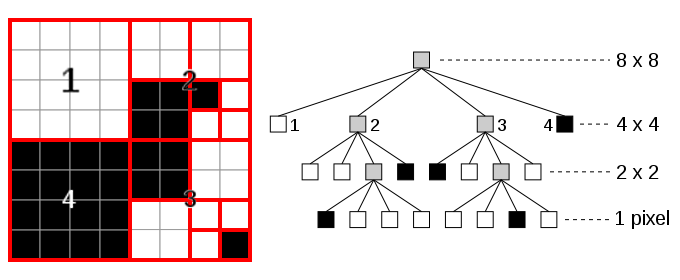
\includegraphics[width=0.6\textwidth]{quadtree.png}
        \vspace{-10pt}
        \captionsetup{justification=centering}
        \caption{Quadtree example on an image of two regions.\\
        Though the image contains 64 pixels, only 21 nodes were used.}
    \end{center}
    \vspace{-25pt}
\end{figure}

\subsection{Methods}
The methods required to operate a quadtree are very similar to the ones of a binary tree. To \textbf{build} the quadtree, start with the largest region and keep breaking it further down. If a node's all four children have an identical value, discard them and set the value to the node, stopping the recursion. Alternatively, one can start with a completely empty image and build the quadtree through repeatedly calling \textit{update}.

\textbf{Querying} the quad tree is done recursively. Start at the top level and work your way down, similar how you would in a binary tree. If querying for a range that consists of multiple regions, split the execution and combine the results.

To \textbf{update}, perform query, but change tree values instead of returning them. If attempting to set part of an unbroken region to a different value, the region needs to be split.`

\subsection{Applications}
While we explored quadtrees in the context of region encoding, we are not limited to performing this narrow task. Quadtrees are structures that are capable of standing on their own as a data structure, and can be applied to so many more things!

We can use quadtrees on raw pixel values. As identical RGB values are infrequent, regions should be unified if their pixels are within a certain threshold, their values set to their internal averages. As such, images can be reduced in memory size while altering pixel values as little as possible - a.k.a. \textbf{lossy compression}.
\begin{figure}[!htb]
    \begin{center}
        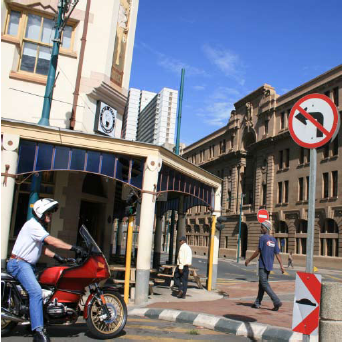
\includegraphics[width=0.275\textwidth]{quadtree_raw.png}
        \hspace{15pt}
        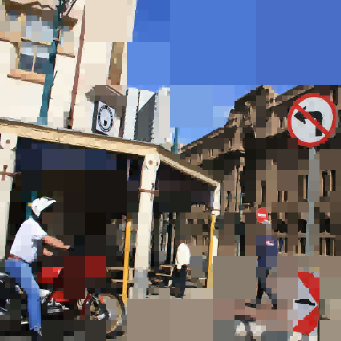
\includegraphics[width=0.275\textwidth]{quadtree_compressed.png}
    \end{center}
    \vspace{-10pt}
    \caption{Quadtree compression}
\end{figure}

Quadtrees aren't limited to images, and can be applied to many tasks that involve values in 2-D regions. Quadtrees can be used to evaluate Excel functions on \textbf{regions of cells}, to solve electromagnetic \textbf{fields}, to speed up \textbf{Conway's Game of Life}. Even problems like \textbf{mesh generation} utilize quadtrees.

Another common type of quadtree problems involves objects placed in continuous space, rather than a grid of values at defined location. These are also called 2-D \textbf{spacial databases}. For example, imagine gas molecules that are trapped in a (2-D) container. We want to \textbf{simulate collisions} between these molecules, but can't afford to check for intersections between every single pair of molecules. Using quad trees, we can split the container into regions that only hold a few molecules each, thus needing to check between fewer pairs.

\section{Image Pyramids}

\subsection{Introduction}

So far, we've mainly focused on transformations that produce images of the same size as the inputs. Oftentimes, however, we want to deviate from the original size - to make images fit on computer screens or make them compatible with printer DPI specifications.

Sometimes it is unclear what the correct output resolution should be. For example, say that we have a model that can detect faces, but it only returns a positive match when the input to it is a 32x32 pixel image centered exactly at the face. If we want to detect faces of different sizes in our scene, we need to shrink or expand it before taking out chunks from it and running them through the model. For convenience, we can stack the different resolutions of our image into an \textbf{image pyramid}, which allows us to make further simplifications and speed up the process.

Pyramids essentially store multiple-resolution copies of an image.  The lowest level of the pyramid is the original image and each layer is 1/4 the size of the previous (half in height and width). 

\subsection{Operations}
Let $g_0$ be the original image $I$ and the lowest layer of the pyramid.  The level $g_l$ is computed by weighted the previous layer values, $g_{l-1}$, with a 5x5 mask ($w$) of weights as follows:

\begin{equation*}
g_l(i,j) = \sum_{m=-2}^{2} \sum_{n=-2}^{2} w(m,n) g_{l-1}(2i+m, 2j+n)
\end{equation*}

Notice how $g_l(i,j)$ references data stored in $g_{l-1}(2i,2j)$, providing intuition for why the size of the pyramid is halved in each dimension. Figure \ref{fig:ImagePyramid} provides a visual for the sequential layer computation. Reduction is the process of "ascending the pyramid" and can be denoted by the $g_l = REDUCE[g_{l-1}]$.

Likewise, we can define an operation to expand the image by a factor of two in each dimension.  We will denote $g_{l,n}$ as the $n^{th}$ expansion of $g_l$.  As such, $g_{l,n} = EXPAND[g_{l,n-1}]$ and $g_{l,0} = g_l$. Don't let the notation confuse you.  All that is happening is that we are adding another subscript to distinguish between a layer in the image pyramid and an image formed from expansion. 

Mathematically, expansion can be done as follows:
\begin{equation*}
g_{l,n}(i,j) = \sum_{m=-2}^{2} \sum_{n=-2}^{2} w(m,n) g_{l,n-1}(\frac{i-m}{2}, \frac{j-n}{2})
\end{equation*}

\begin{figure}
  \centering
    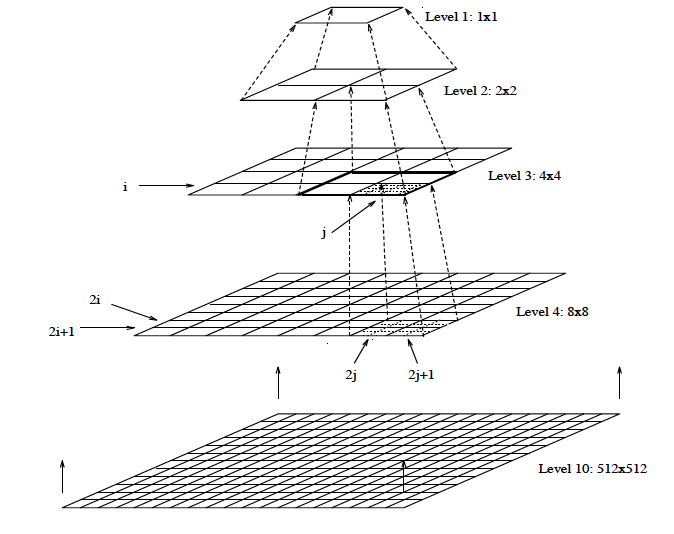
\includegraphics[width=0.5\textwidth]{ImagePyramid.png}
    \vspace{-10pt}
  \caption{Reduction in Image Pyramid}
  \label{fig:ImagePyramid}
  \vspace{-25pt}
\end{figure}

Note that the expressions $\dfrac{i-m}{2}$ and $\dfrac{j-n}{2}$ may not be integers, which is problematic because we are dealing with pixels. The solution is to simply ignore terms that have non-integer pixel locations.  

We chose a mask size of 5, but it is worth noting that all operations can be performed with different mask sizes. 


\subsection{Gaussian Pyramids}
We have defined a general model for image pyramids through operations of expansion and reduction.  Now, we will investigate the properties of the Gaussian Pyramid:
\begin{enumerate}
    \item \textbf{Separability}: In general, Gaussian functions can be written as a product of their uni-variate components.  In other words, the weight mask $w(m,n)$ that we defined in our pyramid operations can be written as a product of some row mask $\hat{w}(m)$ and column mask $\hat{w}(n)$.  Thus, instead of applying a 2-D convolution with $w(m,n)$, we can apply a 1-D convolution with $\hat{w}(m)$ to halve the image width followed by another 1-D convolution with $\hat{w}(n)$ to halve the image height.  The order of applying these two  does not matter.  This reduces the complexity of our operations from $O(N^2)$ to $O(2N)$, which is a significant speedup!
    \item \textbf{Symmetry}: Gaussian functions are symmetric, so the values on end of the mask will be equal to those on the opposite side.  As a result, we can write the 1-D Gaussian vectors as $[c, b, a, b, c]$ and $[c, b, a, b, c]^T$. We can impose two additional constraints to draw relationships between c, b, and a.  
    
    First, the sum of the entire vector vector must be 1. 
    \begin{equation}
        a + 2b + 2c = 1
    \end{equation}
    Second, the total contributions of each pixel's weights for the next layer must be equal. Thus,
    \begin{equation}
        2b = a + 2c
    \end{equation}
    Solving this system of equations, we get a Gaussian mask of $[\frac{1}{4}-\frac{a}{2}, \frac{1}{4}, a, \frac{1}{4}, \frac{1}{4}-\frac{a}{2}]$
    The value of $a$ is subject to parameter tuning and controls the spread of the gaussian function.
\end{enumerate}

Applying a Gaussian function gives us several effects:
\begin{enumerate}
\item It makes the higher levels of our pyramid sample data well from their lower-level creators, and prevents them from appearing coarse due to uneven sampling.
\item It makes our $EXPAND$ function \textbf{apply Gaussian blur} to the layers of the image. If we consider levels of the pyramid as already processed through the Gaussian kernel (upon their creation), $EXPAND$ing blurs them more are creates an image with an apparent \textbf{wider gaussian blur}.
\end{enumerate}

\subsection{Laplacian Pyramids}
\begin{wrapfigure}{r}{0.3\textwidth}
  \begin{center}
    \vspace{-40pt}
    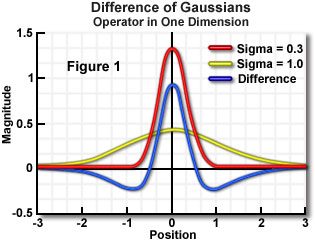
\includegraphics[width=0.30\textwidth]{dog.jpg}
    \vspace{-25pt}
  \end{center}
  \caption{DoG in one dimension}
  \vspace{-20pt}
\end{wrapfigure}

So far, we've created the pyramid, and we've applied $EXPAND$ to every layer of it. We now have $l$ normal images (relatively sharp, narrow Gaussian blur) and $l$ expanded images (blurry, wide Gaissuan blur).

Why do I bring up the width of the kernel? Well, let's take a step back. Recall from the Edge Detection lecture that we can find edges in images by applying the \textit{Laplacian of Gaussian} kernel, which we then found as the second gradient of the Gaussian. As it turns out, we can find a nearly identical kernel through \textbf{Difference of Gaussian}. As the name implies, DoG involves subtracting a wide Gaussian kernel from a narrow Gaussian kernel, which produces the familiar sombrero-like shape.

With this knowledge, we can subtract our expanded images from our regular images, for every layer in the pyramid. What we get is a Laplacian (edge) image for every layer of the pyramid.

\subsection{Applications}
\begin{wrapfigure}{r}{0.375\textwidth}
  \begin{center}
    \vspace{-55pt}
    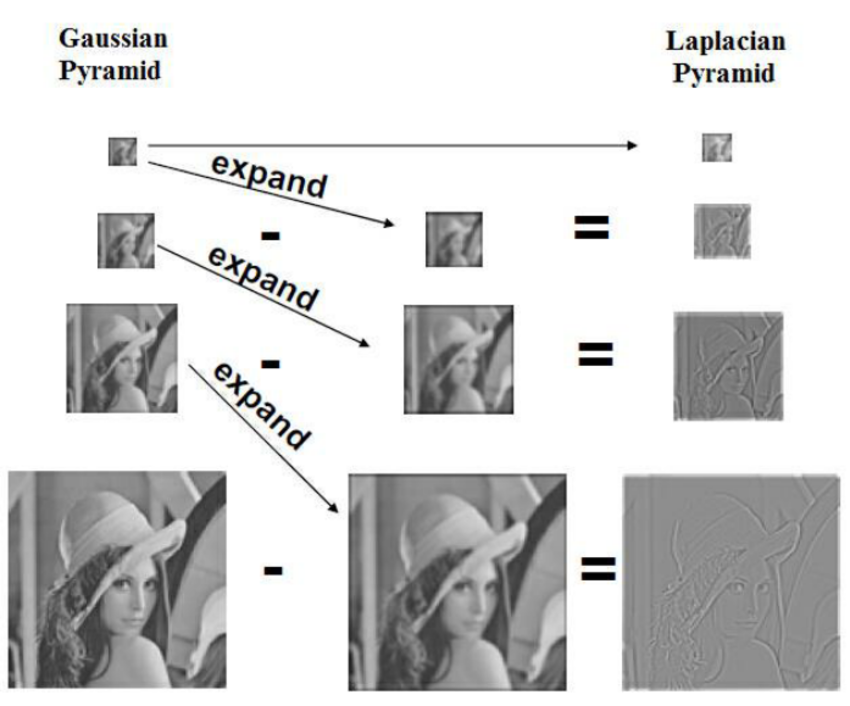
\includegraphics[width=0.375\textwidth]{pyramids.png}
    \hspace{5pt}
    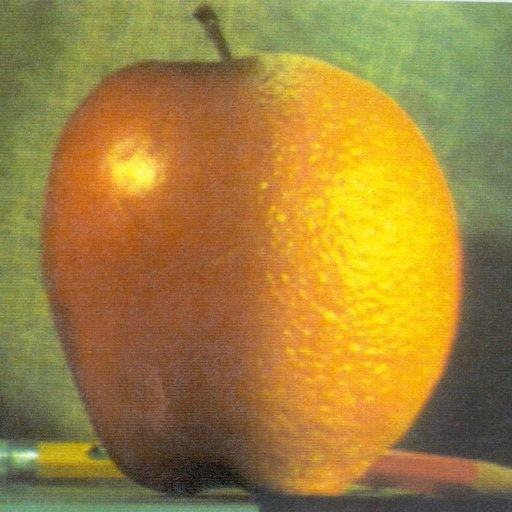
\includegraphics[width=0.225\textwidth]{blended.jpg}
    \vspace{-15pt}
  \end{center}
  \caption{[top] How to obtain Laplacian [bottom] Image-blended Applorange}
  \vspace{-20pt}
\end{wrapfigure}

Okay, but what can we do with this Laplacian pyramid? As it turns out, a really cool practical application is \textbf{image blending}. While it's possible to simply combine two images and blur the seam line, a much prettier result can be obtained by first combining the various levels of their Laplacian Pyramids and then filling those back in.

Sometimes, we are searching an image for a known pattern, a problem known as \textbf{correlation}. We can greatly reduce the number of comparisons required by searching the top layers of the image pyramid before continuing to the lower layers.

As previously mentioned, pyramids can be extensively used when a specific image size is not known. They are often utilized in \textbf{object and face detection}, to detect objects that are both large and small.

Image pyramids can also be useful in applications where the user is panning over a rendered 2-D space, such as Google Maps or when visualizing a fractal. To make the process faster, downsampled versions can be transmitted before their full-size counterparts, and sub-regions of known images can be used when zooming in or out.
\end{document}